\scanpage{14}
% archive sheet number: 13

\deleted{Si $d=-1$ \deleted{ou $d=0$,}\inserted{ou $d=0$} c'est évident. Supposons $d\geq 1$, i.e. $F\ne\varnothing$, on sait que $F$ est l'enveloppe convexe de l'ens de ses pts extrémaux, donc $\exists F'\in\operatorname{Fac}(C)$ \unsure{un|avec} \unsure{dim} $F'=0$, et $F'\deleted{\unsure{\subset|<}}\inserted{\leq}F$, \deleted{\unsure{donc}}\inserted{en fait} $F'<F$.}

$\ast$ \uline{Application à la fonction dimension}

\margin{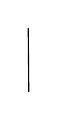
\begin{tikzpicture}[x=1em,y=1em]\draw (0,2.3)--(.02,0);\end{tikzpicture}} \uline{Cor. 4} Soit $C$ un polyèdre convexe, $F_1,\deleted{\unsure{C_2}}F_2\in\operatorname{Fac}(C)$ avec $F_1<F_2$. Pour que $F_2$ soit un \uline{successeur} de $F_1$ (i.e qu'il n'existe pas $F$ tel que $F_1<F<F_2$) il f et s qu'on ait

\[
 \dim F_2=\dim F_1+1
\]

Comme $\dim F$ est fonction \uline{\unsure{strictt|stricte}} croissante sur $\operatorname{Fac}(C)$, la suffisance est claire. Pour la nécessité, \deleted{\unsure{c'est clair si} $\dim F$ \unsure{par}} OPS \inserted{d'abord} $F_2=\deleted{\unsure{F_C|\mathring C}}1$ (plus grande facette), \deleted{et $F_2$} puis en passant au polaire (échange les rôles de $F_1$ et $F_2$) que $F_1=\deleted{\unsure{\varnothing}}0$ (plus petite facette), et à nouveau $F_2=1$. Donc

l'assertion devient maintenant : Pour que il n'existe aucune facette \deleted{\illegible{1}} distincte de $\mathring C$ et de la facette vide, il f et s que $\dim C\unsure{\leq|=}0$ ou $-1$ i.e. que $C$ \inserted{vide ou} réduit à un pt. \deleted{\unsure{car}} (Sinon, en effet, on prend point extrémal !) 

\uline{Cor. 5} La fonction \inserted{$d:F\unsure{\mapsto|\vdash}$} $\dim F$ sur $\operatorname{Fac}(C)$ (du cor. 4) est caractérisée par les conditions

a) $d(F_{\unsure{2|1}})=d(F_1)+1$ si $F_2$ est un successeur de $F_1$

b) $d(\varnothing)=-1$ \margin{\begin{tikzpicture}[x=1em,y=1em]\draw[->] (0,.35) .. controls (0,.02) and (.28,.08) .. (.75,.09);\end{tikzpicture} plus petit él.} De plus $d$ est str. \unsure{croissante|croissant}
